%IMPORTS
\documentclass[a4paper, 11pt]{article}
\usepackage[utf8]{inputenc} 
\usepackage[T1]{fontenc}
\usepackage[catalan]{babel}
\usepackage{amsmath, amssymb, amsthm}
\usepackage[margin=1in]{geometry}
\usepackage{enumerate}
\usepackage{array}
\usepackage{graphicx}
\usepackage{wrapfig}
\usepackage{ragged2e} 
\usepackage{subfig}
\usepackage{caption}
\usepackage{subcaption}
\usepackage[dvipsnames]{xcolor}
%\usepackage[table]{xcolor}
\usepackage{float}
\usepackage{chngcntr}
\usepackage{ragged2e}
\usepackage{multirow}
\usepackage{vmargin}
\usepackage{hyperref}
\usepackage{url}
\usepackage{fancyhdr}
\usepackage{bigints}
\usepackage{listings}
\usepackage{xcolor,colortbl}
\usepackage{subcaption}
%\usepackage{slashbox}

\definecolor{navy}{rgb}{0,0,128}
\definecolor{codegreen}{rgb}{0,0.6,0}
\definecolor{codegray}{rgb}{0.5,0.5,0.5}
\definecolor{codepurple}{rgb}{0.58,0,0.82}
\definecolor{backcolour}{rgb}{0.95,0.95,0.92}
\definecolor{amaranth}{rgb}{0.9, 0.17, 0.31}
\definecolor{GRAY}{rgb}{0.75, 0.75, 0.75}
\definecolor{deepfuchsia}{rgb}{0.76, 0.33, 0.76}
\definecolor{deepmagenta}{rgb}{0.8, 0.0, 0.8}
\definecolor{funcblue}{rgb}{0.36, 0.57, 0.9}
\lstdefinestyle{mystyle}{
    backgroundcolor=\color{white},   
    commentstyle=\color{codegreen},
    keywordstyle=\color{RoyalBlue},
    numberstyle=\tiny\color{codegray},
    stringstyle=\color{codepurple},
    basicstyle=\ttfamily\footnotesize,
    breakatwhitespace=false,         
    breaklines=true,                 
    captionpos=b,                    
    keepspaces=true,                 
    %numbers=left,                    
    numbersep=5pt,                  
    showspaces=false,                
    showstringspaces=false,
    showtabs=false,                  
    tabsize=2
}
\lstdefinestyle{Bash}
{language=bash,
keywordstyle=\color{blue},
basicstyle=\ttfamily,
morekeywords={peter@kbpet},
morekeywords=[2]{make},
keywordstyle=[2]{\color{blue}},
literate={\$}{{\textcolor{blue}{\$}}}1 
         {:}{{\textcolor{blue}{:}}}1
         {~}{{\textcolor{blue}{\textasciitilde}}}1,
}
\lstdefinestyle{BASH}
{language=bash,
keywordstyle=\color{blue},
basicstyle=\ttfamily,
morekeywords={peter@kbpet},
morekeywords=[2]{make},
fontsize=5pt
keywordstyle=[2]{\color{blue}},
literate={\$}{{\textcolor{blue}{\$}}}1 
         {:}{{\textcolor{blue}{:}}}1
         {~}{{\textcolor{blue}{\textasciitilde}}}1,
}

\lstset{style=mystyle}

\setpapersize{A4}
\setmargins{2.5cm}     % margen izquierdo
{2.6cm}                % margen superior
{16.5cm}               % anchura del texto
{23.7cm}               % altura del texto
{10pt}                 % altura de los encabezados
{0cm}                  % espacio entre el texto y los encabezados
{0pt}                  % altura del pie de página
{1cm}                  % espacio entre el texto y el pie de página
\renewcommand{\baselinestretch}{1.5}
\begin{document}

\begin{titlepage}
    \centering
    {\bfseries\LARGE \hspace{1.9em} Universitat Autònoma de Barcelona\newline Facultat de Ciències\par}
    \vspace{2cm}
    {\hspace{-1em}
\includegraphics[width=0.4\textwidth]{logo.png}\par}
    \vspace{1cm}
    {\scshape\Huge Pràctica 4\par} 
    \vspace{1cm}
    {\Large \itshape Autors: \par}
    {\Large \hspace{-1.75em} Gerard Lahuerta \& Ona Sánchez \par}
    {\Large 1601350 --- 1601181 \par}
    \vspace{1cm}
    {\Large 7 de Juny del 2022\par}
\end{titlepage}

\justifying

\newpage
\setcounter{page}{2}
\pagestyle{plain}
\tableofcontents
\cleardoublepage
\addcontentsline{}{chapter}{}
\newpage
\section{Presentació de la llibreria i informació d'interès}
La llibreria de funcions ha estat programada en llenguatge $C$ i consta de dos fitxers, un fitxer capcelera i un amb el codi de la funció.\\
Aquest fitxer amb codi precisa de les llibreries \textcolor{LimeGreen}{math.h} i \textcolor{LimeGreen}{RK4.h}.\\ 
També, el fitxer capcelera té definida la constant:
\begin{itemize}\label{errorrk4}
    \item \textcolor{Dandelion}{E\_STEP}: missatge d'error per valor del nombre de passos inferior o igual a 0.
\end{itemize}
La llibreria té programada únicament la funció \textbf{\textcolor{funcblue}{RK4()}} que permet calcular numèricament el valor d'equacions diferencials mitjançant $n$ passos introduïts amb un \textit{Runge Kutta} d'ordre $4$.\\
Recalcar a més, que la funció conté el seu $CDocs$ propi que conté la informació més rellevant de la funció de manera resumida: \textit{input, output, descripció} i \textit{informació rellevant}.\\ 
\newpage
\section{Presentació dels programes}
\subsection{Fitxer $RK4.c$}
\subsubsection{RK4}\label{muller}
\begin{itemize}
    \item Entrada: 
    \begin{itemize}
        \item[$\circ$] Funció de la variable x: \textbf{\textcolor{Turquoise}{double}}\textbf{\textcolor{deepmagenta}{*}} $f$
        \item[$\circ$] Funció de la variable y: \textbf{\textcolor{Turquoise}{double}}\textbf{\textcolor{deepmagenta}{*}} $g$
        \begin{itemize}
            \item La funció $f$ i $g$ són del tipus: \textbf{\textcolor{Turquoise}{double}}(\textbf{\textcolor{Turquoise}{double}}, \textbf{\textcolor{Turquoise}{double}}, \textbf{\textcolor{Turquoise}{double}}, \textbf{\textcolor{Turquoise}{void}}\textbf{\textcolor{deepmagenta}{*}})
        \end{itemize}
        \item[$\circ$] Valor inicial de x: \textbf{\textcolor{Turquoise}{double}} $x0$
        \item[$\circ$] Valor inicial de y: \textbf{\textcolor{Turquoise}{double}} $y0$
        \item[$\circ$] Valor inicial del temps: \textbf{\textcolor{Turquoise}{double}} $t0$
        \item[$\circ$] Valor final del temps:
        \textbf{\textcolor{Turquoise}{double}} $tf$
        \item[$\circ$] Nombre de passos per fer el Runge Kutta:
        \textbf{\textcolor{Turquoise}{int}} $n$
        \item[$\circ$] Vector de paràmetres necessaris per la funció f: \textbf{\textcolor{Turquoise}{void}}\textbf{\textcolor{deepmagenta}{*}} $prmf$
        \item[$\circ$] Vector de paràmetres necessaris per la funció g: \textbf{\textcolor{Turquoise}{void}}\textbf{\textcolor{deepmagenta}{*}} $prmg$
    \end{itemize}
    \item Sortida: No retorna cap valor, \textbf{\textcolor{Turquoise}{void}}.
    \item Funcionament: Calcula el resultat numèric d'un sistema EDOs de dues variables usant un \textit{Runge Kutta} d'ordre 4. Per trobar els valors $x$ i $y$:
    $$x_{n+1} = x_n + \frac{h}{6}\cdot (k_{n1} + 2k_{n2} +2k_{n3} + k_{n4})$$
    $$y_{n+1} = y_n + \frac{h}{6}\cdot (l_{n1} + 2l_{n2} +2l_{n3} + l_{n4})$$
\end{itemize}
\newpage
\section{Control d'errors}
\subsection{$RK4.c: RK4$}
Per tal d'assegurar el correcte funcionament la funció, es confirmarà la correcta introducció dels paràmetres.\\
Es comprovarà que:
\begin{enumerate}
    \item El valor del paràmere n és major que $0$.
\end{enumerate}
En cas d'inclompir aquesta condició el programa actuarà de la següent manera:
\begin{enumerate}
    \item Es mostrarà per pantalla el missatge d'error corresponent, guardat a la variable \textcolor{Dandelion}{E\_STEPS} (explicada anteriorment a la secció \textcolor{blue}{\textbf{\ref{errorrk4}}}).
    \item No modificarà les variables $x$ i $y$ i finalitzarà inmediatament la funció.
\end{enumerate}

\subsection{$pendol.c$}
Per tal d'assegurar el correcte funcionament del programa i que l'equació que es vol resoldre mantingui el sentit físic, es comprovarà que:
\begin{enumerate}
    \item Els valors introduïts per paràmetre s'han guardat correctament a la variable corresponent.
    \item El valor dels paràmeres $m$ i $L$ son majors que $0$, i $\alpha \geq 0$.
    \item El valor del paràmere $n$ és major que $0$.
\end{enumerate}
En cas d'inclompir alguna d'aquestes condicions el programa actuarà de la següent manera:
\begin{enumerate}
    \item Es mostrarà per pantalla el missatge d'error corresponent i es retornarà un -1.
    \item Es mostrarà per pantalla el missatge d'error corresponent i es retornarà un -2.
    \item Es mostrarà per pantalla el missatge d'error corresponent i es retornarà un -3.
\end{enumerate}

\newpage
\section{Compilació i execució}
\subsection{Compilació del Programa}
\subsubsection{Makefile}
Per facilitar la compilació del programa s'ha creat un fitxer $makefile$ que inclou tant les comandes per crear l'executable com altres comandes associades ($clean$ i $clean\_all$ que explicarem més endavant) per la correcta gestió dels fitxers que s'obtenen de l'execució del makefile.\\
Per compilar el programa i generar l'executable ($pendol$) només cal escriure a la terminal on es troben tots els fitxers (inclós el $makefile$) la comanda make: 
\begin{verbatim}
    $make
\end{verbatim}
Per tal de facilitar la generació del retrat de fase demanat i així comprovar que funcioni correctament, s'ha afegit una opció al makefile per obtenir l'executable que genera un gràfic (el del retrat de fase explicat a \textcolor{blue}{\ref{retrat_fase}}), usant la comanda:
\begin{verbatim}
    $make graphics
\end{verbatim}
Com hem comentat anteriorment, el fitxer makefile també conté comandes per la correcta gestió dels fitxers resultants d'obtenir l'executable, aquestes comandes són:
\begin{verbatim}
    $make clean
    $make clean_all
\end{verbatim}
La comanda $clean$ elimina tots el fitxers $.o$ del directori mentre que la comanda $clean\_all$ elimina tant l'executable com els fitxers amb terminació $.o$.\\
Mencionar que no es poden utilitzar les dues comandes de manera seguida ja que donarà error.\\
\textbf{Important:} en cas de no utilitzar el sistema operatiu $Linux$ (o semblants) o $IOS$ cal modificar la variable $DELETE$ de l'arxiu $makefile$ per a poder utilitzar-lo (substituir per la comanda $del$ en cas d'utilitzar Windows).
\newpage
\subsubsection{Compilació manual}
En cas de voler compilar el programa de manera manual (comanda a comanda) utilitzar en ordre les següents comandes al terminal (una vegada ubicat al directori on es troben els fitxers).
\begin{verbatim}
    $gcc -c RK4.c
    $gcc -c pendol.c  RK4.c -lm
    $gcc pendol.o  RK4.o -lm -o pendol
\end{verbatim}
En cas de voler usar l'executable que genera un gràfic, cal donar-li permisos d'execució, usant les següent comandes:
\begin{verbatim}
    $chmod 744 gnu_graphic.gp
    $chmod 744 generator_graphic.sh
\end{verbatim}
\vspace{1.5em}
\subsection{Execució del Programa}
Adjuntem acontinuació les diferents comandes que hi oferim amb la descripció de cada una:
\begin{table}[h]
    \centering
    \begin{tabular}{l|l}
        \textbf{Comanda} & \textbf{Descripció} \\ \hline \hline 
        \multirow{2}{*}{\texttt{./pendol $\alpha$ $m$ $L$ $x_0$ $y_0$ $t_0$ $t_f$ $n$}} & Genera $n$ valors del sistema $x$, $y$ entre $t_0$ i $t_f$ usant un \\
        &  Runge Kutta d'ordre 4 amb un pas de $100$.\\\hline
        \multirow{2}{*}{\texttt{./generator\_graphics.sh}} & Mitjançant l'executable $pendol$ i $gnu\_graphics.gp$ guarda\\
        & una imatge anomenada $graphic.png$ mostrada a \textcolor{blue}{\ref{retrat_fase}}\\\hline
    \end{tabular}
    \label{tab:my_label}
\end{table}\\
\hspace{-1.5em}Qualsevol argument de més que s'introdueixi al programa serà omés.\\\\

\newpage



\section{Comprovacions de funcionament} \label{comprovacions}
S'han decidit representar els resultats obtinguts mitjançant el programa \texttt{gnuplot} amb les dades obtigudes canviant el valors dels paràmetres i deduïnt si el gràfic obtingut és esperable segons el sentit físic.\\
Mitjançant l'execució del programa \texttt{generador\_graphics.sh} s'obté el retrat de fase d'un cos amb massa $1$ i una llargada de corda de $1$ experimentant diveres velocitats i acceleracions sense fregament. El grafic obtingut és el següent:\\
\begin{figure}[h]
    \centering
    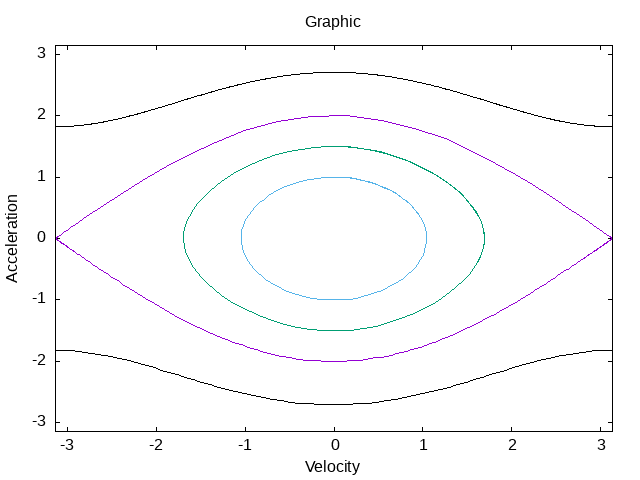
\includegraphics[width = 0.8 \textwidth]{ojoxd.PNG}
    \caption{Retrat de Fase del sistema per als valors $(\alpha, m, L) = (0, 1, 1)$}
    \label{retrat_fase}
\end{figure}
\\
Com s'observa, el gràfic té un sentit físic esperable ja que:
\begin{enumerate}
    \item Si l'objecte comença amb una velocitat petita i no amb la suficient acceleració (es troba dins de la regió delimitada per les línies liles) l'objecte oscil·larà at infinitum. Això es reflexa fent que les corbes de nivell siguin tancades, no tendeixin a cap valor i reflexant que quan la velocitat és màxima (en mòdul) l'acceleració és $0$ i que quan l'acceleració és màxima (en mòdul) la velocitat és $0$.
    \item Si l'objete inicia amb la velocitat exacta i/o amb l'acceleració necessària com per trobar-se sobre la linia de color lila, l'objecte rota amb l'energia necessària com per a arribar a la part més alta de la circumferència que traça amb velocitat $0$. Aquest fenòmen (similar al primer cas) es manifesta gràficament com una ona cosenoïdal.
    
    \item Si a l'objecte se li dona una acceleració inicial suficient (es troba per fora de la regió delimitada per les linies liles) l'objecte donarà infinites voltes arribant a la part més alta de la trajectoria amb una velocitat i acceleració diferent de $0$. Aquest fenòmen es representa gràficament com una ona cosenoïdal similar al segon cas però desplaçada en l'eix d'ordenades reflexant que l'acceleració mai valdrà $0$.
\end{enumerate}
Per altre anda, si hi afegim una força de fregament, obtenim el següent gràfic:\\
\begin{figure}[h]
    \centering
    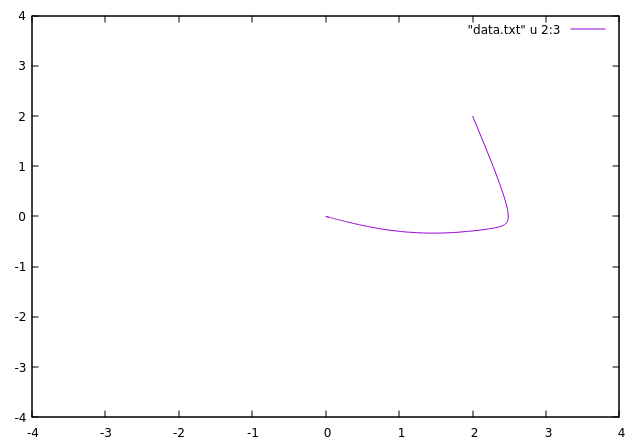
\includegraphics[width = 0.8 \textwidth]{codo.png}
    \caption{Retrat de Fase del sistema per als valors $(\alpha, m, L,x_0,y_0) = (3,1,1,2,2)$}
    \label{retrat_fase}
\end{figure}\\
S'observa d'aquí que tant l'acceleració com la velocitat tendeixen a anar cap a 0 (i de manera bastant ràpida) degut a que l'acceleració generada per la força de fregament és major que la que hi tenim inicialment.
\newpage
\hspace{-1.5em}Per altra banda, cal mencionar que si la introducció dels paràmetres no es fa amb cura i s'introdueixen valors de temps massa grans sense reajustar el valor d'intervals a calcular el programa pot no donar resultats correctes; per exemple en aquest cas:
\begin{figure}[h]
 \centering
  \subfloat[$(t_f,n) = (10^8,10^3)$]{
    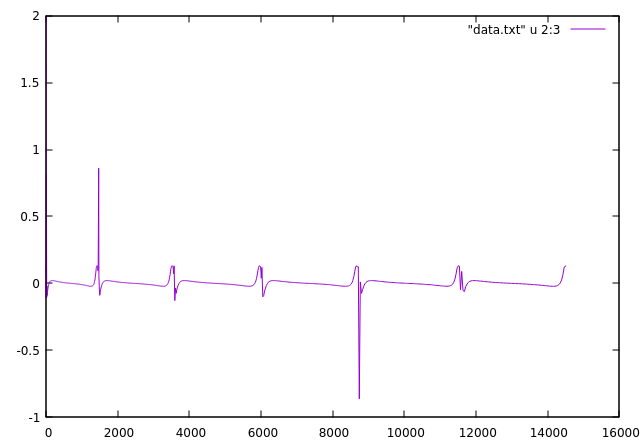
\includegraphics[width=0.5\textwidth]{picosraros.png}}
  \subfloat[$(t_f,n) = (10^4,10^5)$]{
    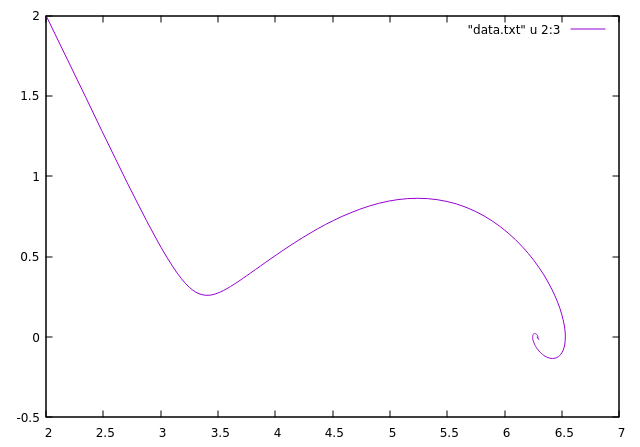
\includegraphics[width=0.5\textwidth]{curbita.png}}
    \caption{Gràfics generats per al sistema $(\alpha, m, L,x_0,y_0,t_0) = (2,1,1,2,2,0)$}
\end{figure}
\newpage
\section{Conclusions}
Finalitzem l'informe confirmant (a partir de les comprovacions de funcionament dutes a terme a l'apartat \textcolor{blue}{\ref{comprovacions}}) que el programa $pendol.c$ funciona de manera correcta, proporcionant els valors $x$ i $y$ al llarg d'un cert període de temps, resultants d'un sistema EDOs de dues variables que es resol de forma numèrica usant el mètode Runge Kutta d'ordre 4.\\
També, arrel de les comprovacions dutes a terme a l'apartat mencionat anteriorment, confirmem que el programa $generator\_graphics.sh$ funciona correctament, proporcionant l'exemple de retrat de fase ja explicat.\\

\subsection{Informació adicional}
\begin{itemize}
    \item  La complexitat del mètode és d'ordre lineal; és a dir, $O(n)$ (on $n$ és el nombre de intervals que volem que utilitzi programa).

   \item Responem a la pregunta: \textbf{Quin paper juga el paràmetre $\alpha$?}\\
   A l'equació del pèndol esmorteït $x'' + \alpha x' + \frac{m}{L}sin(x) = 0$, el paràmetre $\alpha$ representa la força de fricció.
   
   
   \item Responem a la pregunta: \textbf{Si $\alpha = 0$, $m=1$ i $L=1$, intenteu obtenir el retrat de fase (gràfic en $x$ i $y$) del pèndol.}\\
    S'ha respòs aquesta pregunta a l'apartat \textcolor{blue}{\ref{comprovacions}}.
   
   \newpage
   
  \item Responem a la pregunta: \textbf{Pel cas $\alpha=0$, $m=1$ i $L=1$, els punts $((2k+1)\pi, 0)$, $k\in \mathbb{Z}$ són selles, i per tant inestables. Què passa si integreu el sistema amb condició inicial en un d'aquests punts amb $t_f$ diferent?}\\
  
  \begin{figure}[h]
 \centering
 \begin{subfigure}
  \subfloat[$t_f = 200$]{
    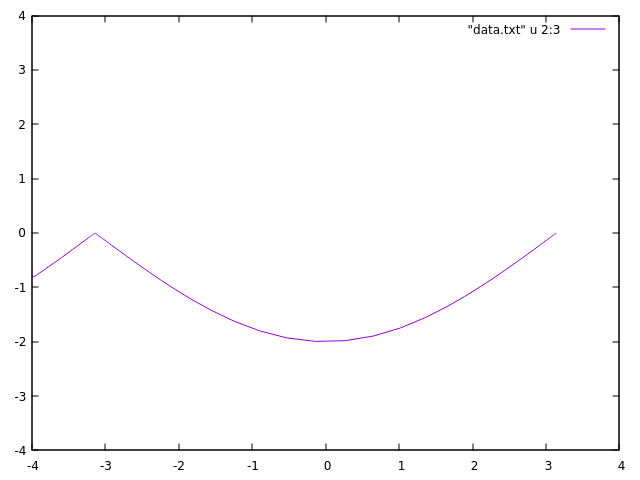
\includegraphics[width=0.465\textwidth]{sella1.png}}
  \subfloat[$t_f = -200$]{
    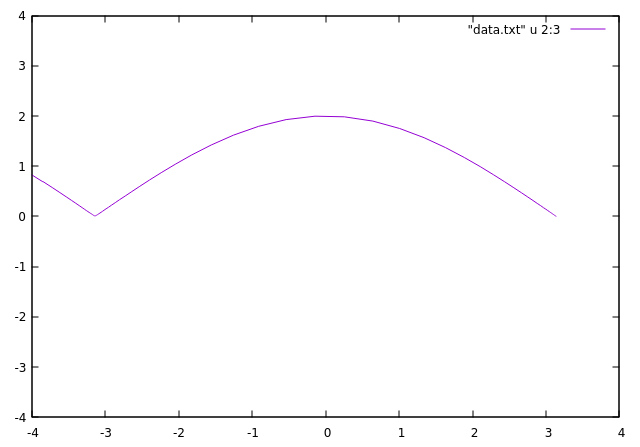
\includegraphics[width=0.5\textwidth]{sella2.png}}
    $$(\alpha, m, L, x_0, y_0, t_0, n) = (0, 1, 1, 3.14, 0, 0, 1000)$$
 \end{subfigure}
 \vspace{-2em}
 \end{figure}
  \begin{figure}[h]
\begin{subfigure}
 \centering
  \subfloat[$t_f = 200$]{
    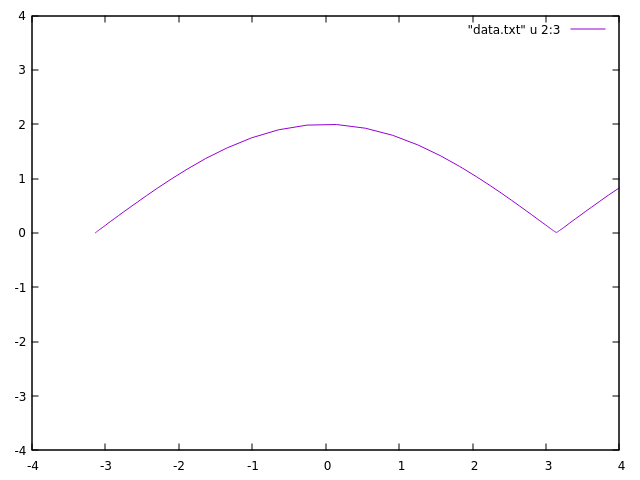
\includegraphics[width=0.465\textwidth]{sella3.png}}
  \subfloat[$t_f = -200$]{
    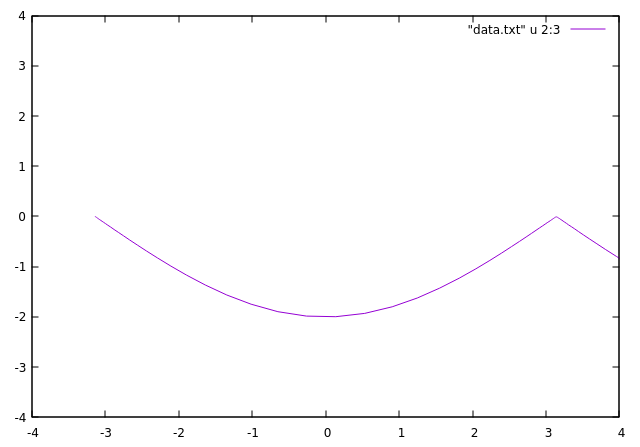
\includegraphics[width=0.5\textwidth]{sella4.png}}
    $$(\alpha, m, L, x_0, y_0, t_0, n)  = (0, 1, 1, -3.14, 0, 0, 1000)$$
\end{subfigure}
\end{figure}
\newpage
\begin{figure}[h]
\begin{subfigure}
 \centering
  \subfloat[$t_f = 10$]{
    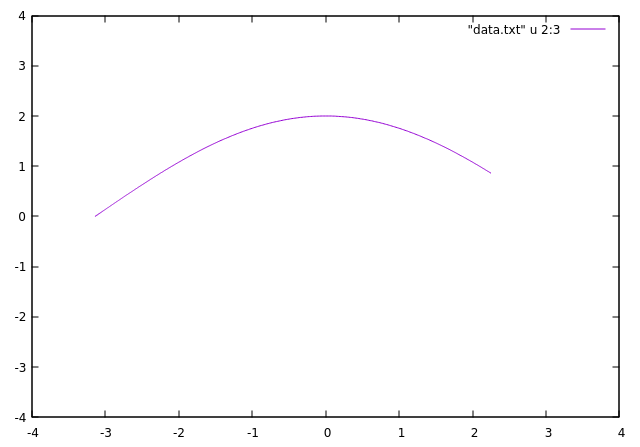
\includegraphics[width=0.465\textwidth]{sella5.png}}
  \subfloat[$t_f = 5$]{
    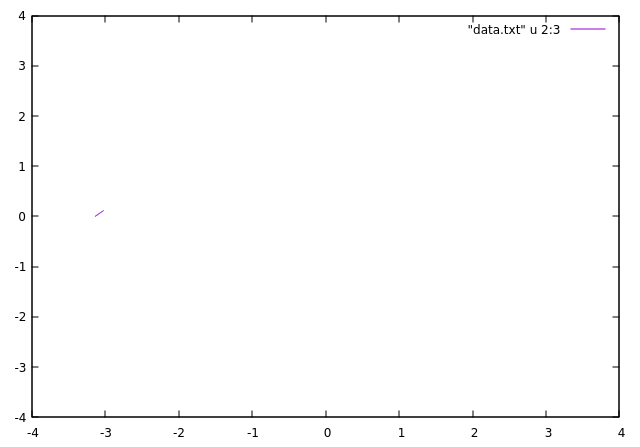
\includegraphics[width=0.5\textwidth]{sella6.png}}
    $$(\alpha, m, L, x_0, y_0, t_0, n)  = (0, 1, 1, -3.14, 0, 0, 1000)$$
\end{subfigure}
\end{figure}\\
Observem comparant el recorregut dels últims dos gràfics amb els anteriors que, canviant el valor del temps el recorregut linea canvia radicalment, en comparació amb els 4 gràfics anteriors.\\
Es dedueix que hi existeix un periode en que la velocitat no varia molt davant el temps transcorrit i una altre on hi augmenta molt (procès al que arriba a la velocitat màxima).\\
Aquest fenòmen correspon al fet que l'acceleració gravitatoria no accelera de la mateixa manera el pendòl en posicions diferents, només accelera una de les dues components del sistema, pel que l'acceleració que hi pateix l'objecte a l'hora d'oscil·lar no varia de forma lineal sino seguint un sinus.
\begin{figure}[h]
    \centering
    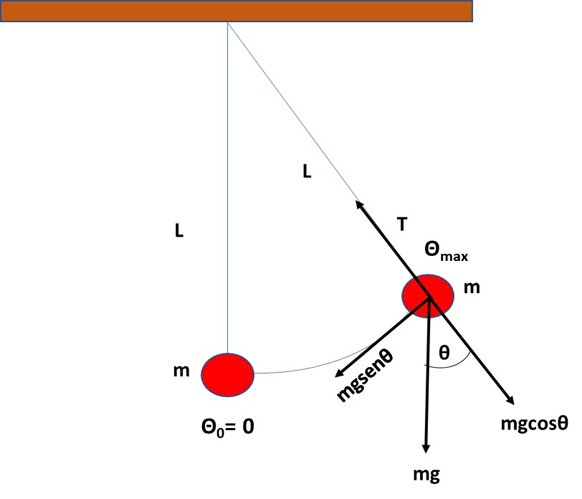
\includegraphics[width = 0.45\textwidth]{pendulo.png}
    \caption{Diagrama de Sòlid Lliure d'un pendòl simple}
    \label{fig:my_label}
\end{figure}


\end{itemize}
\end{document}
